\documentclass[11pt]{article}


\usepackage{amsmath}
\usepackage{textcomp}

% Add other packages here %
\usepackage{graphicx}  
\usepackage{geometry}
 \geometry{
 a4paper,
 left=35mm,
 top=35mm,
 right=35mm,
 bottom=35mm
 }


% Put your group number and names in the author field %
\title{\bf Excercise 4\\ Implementing a centralized agent}
\author{Group \textnumero 3 : Robin \textsc{Clerc}, Pierre \textsc{Vigier}}


% N.B.: The report should not be longer than 3 pages %


\begin{document}
\maketitle

\section{Solution Representation}

\subsection{Variables}
% Describe the variables used in your solution representation %
Our solution is described by an array of length $N_{Vehicles}$ mapping each vehicle to the ordered list of its actions which are represented by a class $MyAction$, .

One $MyAction$ object is described by
\begin{itemize}
    \item a Logist $Task$
    \item the information whether it is a pickup or a delivery
\end{itemize}
There are $2 \times N_{Tasks}$ such action to dispatch on the vehicles set. We can remark that one of those actions represents several actual actions for the agent. This representation is far more convenient to deal with constraints.

\subsection{Constraints}
% Describe the constraints in your solution representation %

By constructing the neighbors of a plan, we are going to generate a lot of invalid plans that we should detect to keep only the valid ones to chose the best neighbor.

The constraints to get a valid plan are :
\begin{itemize}
    \item At each time the load of each vehicle cannot be greater than its capacity.
    \item A vehicle can pickup a task only if it did not have already been taken by a vehicle
    \item A vehicle can deliver a task only if it already carries the task to deliver.
    \item All the tasks must be delivered at the end : the number of actions done by all the vehicles must be $2 \times N_{Tasks}$
\end{itemize}


\subsection{Objective function}
% Describe the function that you optimize %

In this problem we have a fixed set of tasks, thus a fixed global award and we want to generate the maximum profit from this situation. Hence the optimal solution is the one with the minimal cost. Consequently, the objection function is the cost of the plan, that we want to minimize.

The cost of the plan is defined by the sum of the costs of the plans of all the vehicles : $cost = \sum\limits_{k=1}^{N_{Vehicles}}{distanceTravelled(v_k) \times costByKm(v_k)}$.

%With an infinite number of task we could also choose to minimize the duration of the whole delivery to maximize the profitability

\section{Stochastic optimization}

\subsection{Initial solution}
% Describe how you generate the initial solution %

Our initial solution is obtained by giving all the tasks to the vehicle with the highest capacity.

\subsection{Generating neighbours}
% Describe how you generate neighbors %
To generate neighbors we have several operations :
\begin{itemize}
    \item The \textit{intraChanges} : We change the order of actions inside a vehicle. The vehicle has a number of actions $n$ and we select randomly a number $m$ between $0$ and $n$ to choose the number of swaps. Then for each swap we randomly choose the two $MyAction$ objects to swap.
    \item The \textit{interChanges} : For each vehicle we try to give each task (i.e. the two $MyAction$ objects associated) to each other vehicle and apply intraChanges in the destination vehicle to shuffle the actions.
\end{itemize}

\subsection{Stochastic optimization algorithm}
% Describe your stochastic optimization algorithm %

In each iteration of our algorithm we generate neighbors by applying \textit{intraChanges} and \textit{interChanges} to our current solution. 

Then we select the neighbor with the minimal cost. If it is better than the current plan, it becomes the current plan. Otherwise, it becomes the current plan anyway with probability $p$ to avoid getting stuck in local minimum. However we always remember our best plan so far and also have a probability $p'$ to return to this state to avoid getting lost in a dead-end.

Finally, we return the best plan we have ever seen.

By default, we have set $N_{iterations} = 1000$ to prevent from timeout. But to be sure to converge and reach a near optimal solution, we should set $N_{iterations} = 10000$.

\section{Results}

\subsection{Experiment 1: Model parameters}
% if your model has parameters, perform an experiment and analyze the results for different parameter values %

\subsubsection{Setting}
% Describe the settings of your experiment: topology, task configuration, number of tasks, number of vehicles, etc. %
% and the parameters you are analyzing %

We use the English topology, the company A with the four given vehicles and 30 tasks.

We choose to study the impact of the probability $p$ of choosing the best neighbor even if the current state is better. This parameter should control the trade-off between exploration and optimization.

We fix $N_{iterations} = 10000$ so that the algorithm converges i.e. the best cost has not improved for a large number of iterations.

\subsubsection{Observations}
% Describe the experimental results and the conclusions you inferred from these results %

In the figure \ref{trade_off_exploration_optimization}, we can see the cost of the best plan returned by the algorithm for different values of $p$.

\begin{figure}[h!]
\begin{center}
\begin{tabular}{cc}
\begin{minipage}[c]{0.3\linewidth}
\centering
\begin{scriptsize}
\begin{tabular}{|c|c|}
\hline
$p$ & cost \\
\hline
0.0 & 21846 \\
\hline
0.1	& 20187.5 \\
\hline
0.2	& 21859.5 \\
\hline
0.3	& 16758.5 \\
\hline
0.4	& 18151.5 \\
\hline
0.5	& 17861 \\
\hline
0.6	& 19677 \\
\hline
0.7	& 16654 \\
\hline
0.8	& 21676.5 \\
\hline
0.9	& 23829.5 \\
\hline
1.0 & 25144 \\
\hline
\end{tabular}
\end{scriptsize}
\end{minipage}
&
\begin{minipage}[c]{0.5\linewidth}
\centering
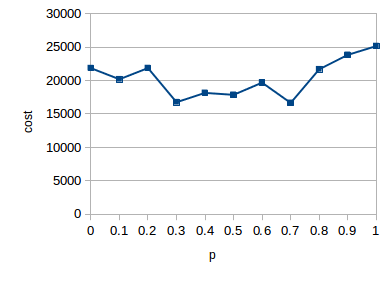
\includegraphics[scale=0.6]{trade_off_exploration_optimization.png}
\end{minipage}
\end{tabular}
\end{center}
\label{trade_off_exploration_optimization}
\end{figure}

These results are not very accurate because we only did one run for each value of $p$. It would have been better to compute an average over several runs. 

However we can already observe a trend. When $p$ is too low that is when we optimize a lot but do not explore much or when $p$ is too high that is when we explore a lot but do not optimize much, the results are worse than when $p$ has an intermediate value. There is really a trade-off.

Finally, according to these results, we set $p = 0.5$.

\subsection{Experiment 2: Different configurations}
% Run simulations for different configurations of the environment (i.e. different tasks and number of vehicles) %

\subsubsection{Setting}
% Describe the settings of your experiment: topology, task configuration, number of tasks, number of vehicles, etc. %

We keep the English topology but we now set the number of tasks to 50 and the number of vehicles to 12.

\subsubsection{Observations}
% Describe the experimental results and the conclusions you inferred from these results %
% Reflect on the fairness of the optimal plans. Observe that optimality requires some vehicles to do more work than others. %
% How does the complexity of your algorithm depend on the number of vehicles and various sizes of the task set? %

The best plan we obtain has a cost of $32524.0$ but what interests us is the repartition of tasks between the vehicles :

\begin{table}[h!]
\centering
\begin{scriptsize}
\begin{tabular}{|c|c|c|c|c|c|c|c|c|c|c|c|c|}
\hline
Vehicle & 1 & 2 & 3 & 4 & 5 & 6 & 7 & 8 & 9 & 10 & 11 & 12 \\
\hline
Number of tasks & 23 & 3 & 4 & 0 & 0 & 6 & 4 & 4 & 6 & 0 & 0 & 0 \\
\hline
\end{tabular}
\end{scriptsize}
\end{table}

We observe that the first vehicle has nearly half of the tasks while 5 vehicles have no tasks at all. Thus while it is good this plan is not fair at all.

The algorithm does not scale very well because the number of neighbors generated at each iteration is $O(N_{vehicles}N_{tasks})$ by performing \textit{interChanges} and $O(N_{tasks}^2)$ by performing \textit{intraChanges}. 

We could fix the complexity of each iteration by setting $N_{intraChanges}$ the number of \textit{intraChanges} and $N_{interChanges}$ the number of \textit{interChanges} we want to perform and then choosing the vehicles and tasks randomly in the corresponding procedures.

\end{document}